\documentclass[8pt]{beamer}
\usepackage[english]{babel}
\usepackage[utf8]{inputenc}
\usepackage[T1]{fontenc}
\usepackage{lmodern}
\usetheme{Warsaw}
\useoutertheme{infolines} 
\setbeamertemplate{items}[ball]
\usepackage{algorithm}
\usepackage{fancybox}
\usepackage{hyperref}
\usepackage{tikz}
\usetikzlibrary{automata,calc,er}
\usetikzlibrary{mindmap,scopes,arrows,arrows.meta,shapes,chains,positioning,fit,backgrounds,decorations,intersections,petri,decorations.pathmorphing}
\usepackage{pgf}
\usepackage{pgfplots}
\pgfplotsset{compat=1.13}
\usetikzlibrary{pgfplots.fillbetween}
\pgfdeclarelayer{ft}
\pgfdeclarelayer{bg}
\pgfsetlayers{bg,main,ft}
\usepackage{graphics}
\usepackage{amssymb}
\usepackage{adjustbox}
\usepackage{wasysym}
\usepackage{siunitx}
\usepackage{makecell}
\usepackage{kbordermatrix}
\usepackage{mathtools}
\usepackage{calc}
\usepackage{fp}
\usepackage{docmute}
\usepackage{graphicx}
\graphicspath{{figures/}}
\tikzstyle{block} = [rectangle, draw, fill=blue!20, 
    text width=6em, text centered, rounded corners, minimum height=4em]
    \tikzstyle{line} = [draw, -latex']
\newcommand<>{\transp}[1]{\fill [draw=none, fill=white, fill opacity=0.7] (#1.north west) -- (#1.north east) -- (#1.south east) -- (#1.south west) -- (#1.north west) -- cycle;}
\begin{document}
\begin{frame}{Problematics}
    \begin{tikzpicture}[line,>=stealth]
        \onslide<+->{\node [label=above:{Real system dynamics}] (realSys) { 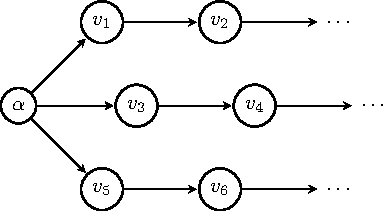
\includegraphics[scale=0.5]{realSystem.pdf}};
        }
        \only<+>{\node [below = of realSys,label=below:{Partial observation}] (partObs) {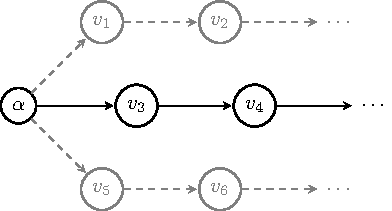
\includegraphics[scale=0.5]{partialObservation.pdf}};
        \draw [dashed,->] (realSys) -- (partObs);
        }
        \onslide<+->{\node [below = of realSys,label=below:{Time series data}] (partObs) {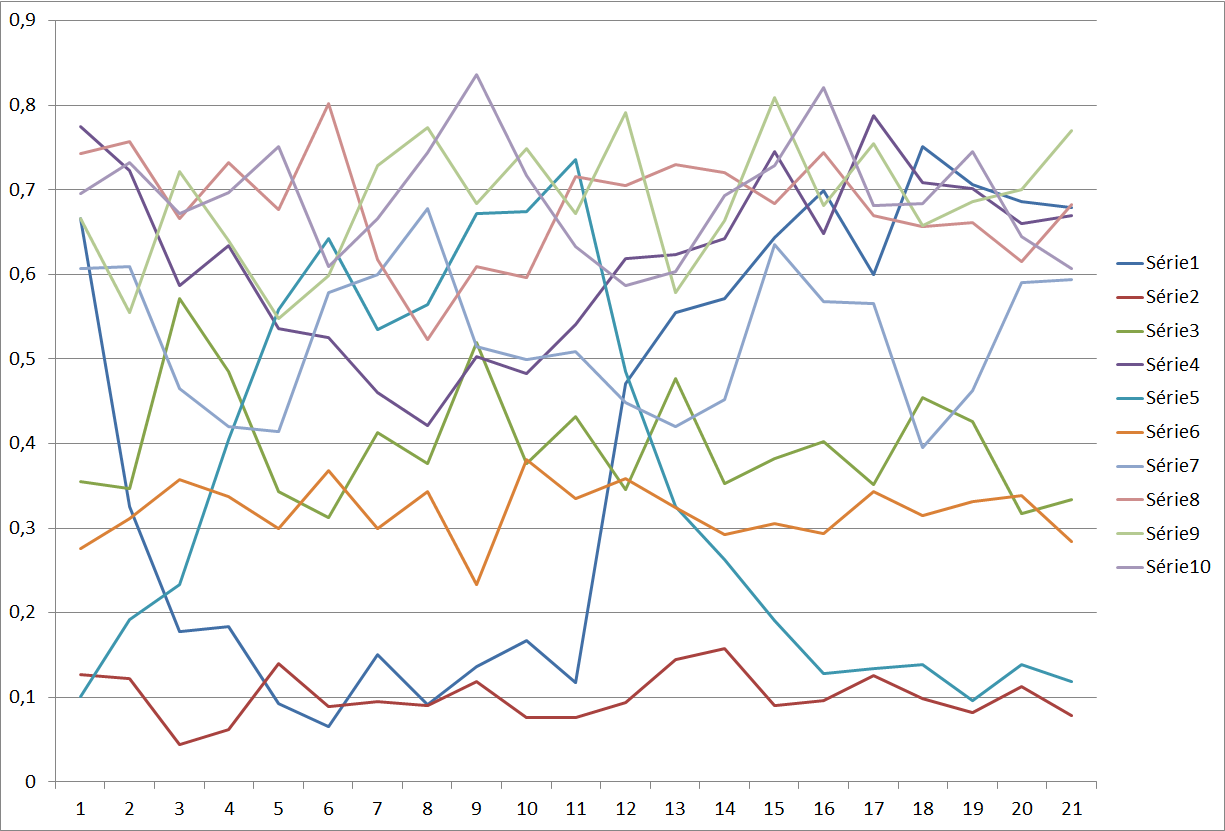
\includegraphics[scale=0.1]{tsd.png}};
        \draw [dashed,->] (realSys) -- (partObs);
        }
        \onslide<+->{\node [right = 1.5cm of partObs,label=below:{Biological regulatory network}](brn){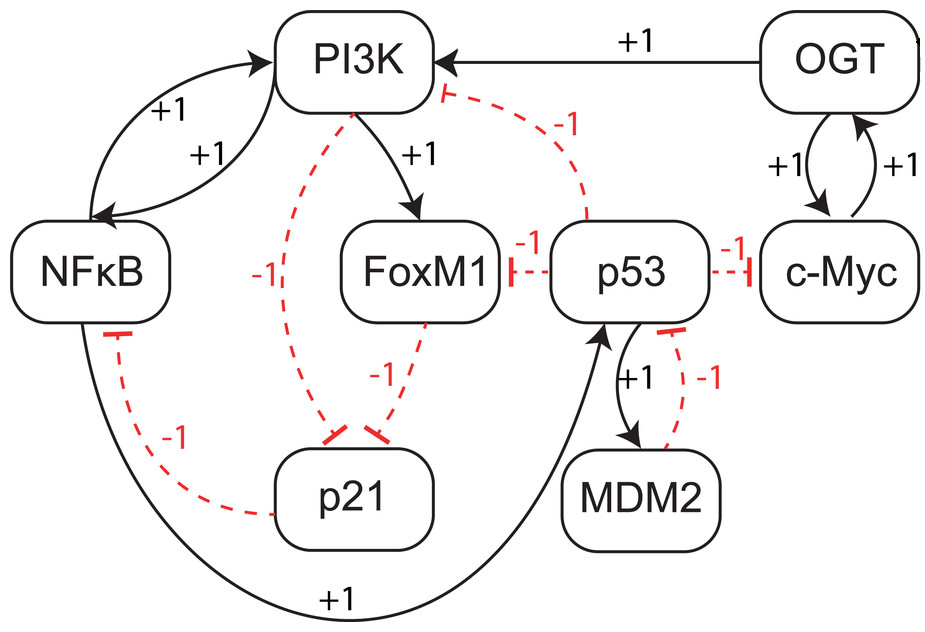
\includegraphics[scale=0.15]{brn.png}};
        \draw [->,color=blue] (partObs) -- node [above,midway] (learning) {Learning} (brn);
        }
        \onslide<+->{\draw [->,thick,color=blue!50] (brn) to node [below left,midway] {\textbf{Reproducible?}} (realSys);}
        \onslide<+->{\node [right = of realSys,label=above:{Biological \textit{a priori} knowledge}] (bioNet) {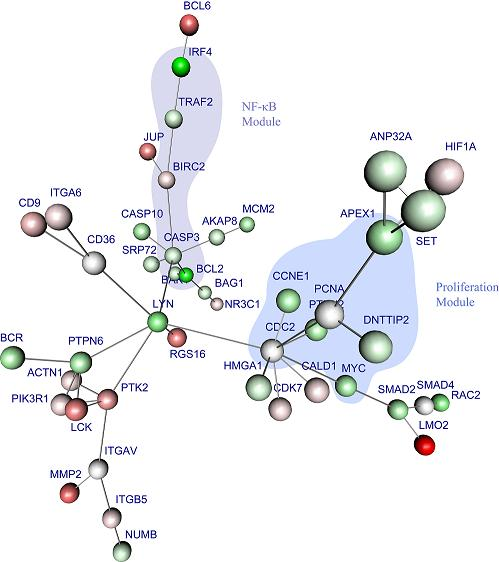
\includegraphics[scale=0.2]{biologicalNetwork.jpg}};
        \draw [dashed,->] (realSys) -- (bioNet);
        }
        
        \onslide<+->{\node [color=blue,right = of bioNet,label=above:{Reachability properties}] (reach) {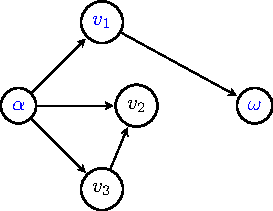
\includegraphics[scale=0.7]{reachability.pdf}};
        \draw [dashed, ->] (bioNet) -- (reach);
        }
        \onslide<+->{\draw [->,color=red] (brn) edge[bend left] node [below right,near start] (modelCheck) {Model Checking} (reach);}
        
        \onslide<+->{\draw [->,color=blue] (reach) edge[bend left] node [below right,midway] (revising) {Revising} (brn);}
        \onslide<+->{
        \transp{realSys}
        \transp{partObs}
        \transp{bioNet}
        \node[draw,ellipse,thick,color=yellow,fit=(modelCheck) (revising),label=below right:\textbf{My work}] (work){};
        }
        \onslide<+->{
            \draw[->,color=blue] (current bounding box.south east)
            ++(-6em, 0em) -- ++(2em, 0)
            node[right] {Inference};
            \draw[->,color=red] (current bounding box.south east)
            ++(-6.5em, 2em) -- ++(2em, 0)
            node[right] {Validation};
        }
    \end{tikzpicture}
\end{frame}
\end{document}
